\documentclass{article}
\usepackage[utf8]{inputenc}
% \usepackage[english]{babel} % disabled to avoid missing language files in TinyTeX; not critical for this manuscript
\usepackage[T1]{fontenc}

% Graphics and figures
\usepackage{graphicx}
\DeclareGraphicsExtensions{.pdf,.png,.jpg}

\usepackage{caption}
\captionsetup{font=small,labelfont=bf,justification=raggedright,singlelinecheck=false, width=0.95\textwidth}

\usepackage{fancyvrb}
\usepackage{authblk}
\usepackage{hyperref}
\usepackage{pdflscape}
\usepackage{setspace}
\usepackage{lineno}
\usepackage{cite}
\usepackage{float}

% TikZ
\usepackage{tikz}
\usetikzlibrary{shapes.geometric, arrows.meta, positioning, calc, external}

% other packages
\usepackage{rotating} % for sidewaystable
\usepackage{chemformula}
\usepackage{siunitx}
\usepackage{palatino}
\usepackage{multirow}
\usepackage{dcolumn}
\usepackage{booktabs}
\usepackage{algorithmic}
\usepackage{pdfpages}
\usepackage{listings}
\usepackage{inconsolata}
\usepackage[final]{microtype} % improved kerning and line breaking

% TikZ styles for flowcharts
\tikzset{
	startstop/.style={ellipse, draw, fill=blue!10, text centered, minimum width=2.4cm, minimum height=0.9cm, font=\footnotesize},
	process/.style={rectangle, draw, fill=orange!20, text centered, minimum width=3.0cm, minimum height=0.9cm, font=\footnotesize},
	decision/.style={diamond, draw, fill=green!20, text centered, aspect=2, minimum width=2.5cm, inner sep=1pt, font=\footnotesize},
	arrow/.style={->, thick, >=stealth}
}

%----------------------------document----------------
\begin{document}
\setkeys{Gin}{width=0.99\textwidth}
% Removed global page background logo; it will be shown only in the Acknowledgements section.
%---------------------------title-------------------
	\title{Retrospective Benchmark of Optical Surface Roughness Workflows Against an Internal Tactile Baseline Across Multiple Materials and Processes}
%---------autorzy--------------------------------------------
\author[1,$^*$]{Dawid~Kucharski}
%\author{}
\author[2]{Piotr~Niesłony}
\author[2]{Jolanta~Królczyk}
\author[2]{Grzegorz~Królczyk}
\author[3]{Katarzyna~Nicińska}
\author[3]{Natalia~Wojciechowska}
\author[3]{Łukasz~Ślusarski}%
\author[1]{Michał~Wieczorowski}
\author[1]{Bartosz~Gapiński}
\affil[1]{Poznan University of Technology, Poland}
\affil[2]{Opole University of Technology, Poland}
\affil[3]{Central Office of Measures, Poland}
\affil[$^*$]{\href{mailto:dawid.kucharski@put.poznan.pl}{dawid.kucharski@put.poznan.pl}}
\vspace{-5mm}
\date{\today\\\vspace{2mm}}
\maketitle
%-------------------abstract---------------------------
\doublespacing
%\linenumbers
\begin{abstract}
This paper presents a retrospective benchmark of optical surface-texture workflows against an internal tactile baseline across six engineering materials and multiple surface-generation processes. Eight profile roughness parameters were analysed. Optical--tactile discrepancy depended strongly on workflow choice. Under the best system--illumination combinations available in the archive, the lowest median discrepancies were obtained for amplitude parameters such as $R_t$, $R_v$, $R_z$, and $R_{z1max}$, whereas $R_{sm}$ remained challenging. Across the strictly positive parameters, tactile repeatability was generally smaller than the observed between-workflow discrepancies, with a median relative standard error of 1.45\%. A fixed-configuration sensitivity analysis showed that the best single workflow with complete archive coverage had a median discrepancy of 24.8\%, quantifying the optimism introduced by per-group retrospective selection. These results support the use of the archive as a practical benchmark for identifying candidate optical configurations for follow-up validation. Because the dataset is retrospective and comparison was possible only for matched exported parameter labels, the study should be interpreted as a workflow-level benchmark rather than as a formal optical--tactile equivalence assessment.

\noindent{\bf Keywords:} surface metrology; optical measurement; tactile reference; surface roughness; illumination wavelength; benchmarking; uncertainty.
\end{abstract}

\section{Introduction}\label{sec:intro}
Surface-texture measurement remains central to manufacturing because reported roughness parameters directly influence process control, specification compliance, and product traceability. In industrial practice, acceptance criteria are still commonly anchored to profile parameters such as $R_a$, $R_q$, $R_{sk}$, $R_{sm}$, $R_t$, $R_v$, $R_z$, and $R_{z1max}$. Tactile stylus profilometry therefore retains practical authority as a reference workflow, even though it is slower, access-limited, and potentially intrusive on delicate or highly finished surfaces.

Recent work has improved both tactile and optical instrumentation, but in different ways. Imkamp et al. described navigator scanning as a route to higher-throughput tactile acquisition without sacrificing the scanning role of stylus metrology~\cite{Imkamp2004165}. Linz et al. presented 3D fibre probes that combine tactile contact with optical read-out and very low probing force~\cite{Linz2012}. M\'inguez-Mart\'inez et al. reported interlaboratory comparison results that are directly relevant to profile-metrology comparability across implementations~\cite{mínguezmartínez2022results-794}. Boedecker et al. showed that white-light interferometer data require transfer-characteristic control and uncertainty-aware comparison before they can be meaningfully related to tactile results~\cite{Boedecker2010}. These developments expand the metrology toolbox, but they do not remove the central comparability problem: optical and tactile systems do not necessarily interrogate the same effective measurand.

That problem has been recognised repeatedly. Dierke and Tutsch showed that the material under test can itself bias optical results, particularly for transparent surfaces~\cite{Dierke2015770}. Tiziani et al. argued that microstructure measurement and description must account for material-specific optical behaviour~\cite{Tiziani1999429}. Garc\'ia et al. compared contact stylus and confocal microscopy methods and showed that precision, accuracy, and algorithmic complexity depend on the chosen workflow~\cite{Garcia2018}. Schmidt et al. compared areal and profile methods for machined components and highlighted that parameter validity can shift with application and material~\cite{Schmidt2021459}. Nouira et al. built a high-precision profilometer precisely to compare tactile and optical measurements of standards under a controlled metrological frame~\cite{Nouira2014a}. Hoefling et al. then showed from an industrial perspective that large object size, reflective surfaces, contamination, and cycle-time demands can become hard method-selection constraints~\cite{Hoefling1999338}. Stavroulakis et al. made the additional point that data fusion and algorithmic post-processing can materially change the final metrological output~\cite{Stavroulakis2020187}. The practical question is therefore not whether optical methods are generally faster or more modern, but under which material--process conditions a given optical workflow remains acceptably close to an established tactile baseline.

Workflow behaviour may also vary with illumination and reconstruction strategy. Hu et al. developed a line-scanning chromatic confocal sensor specifically for highly reflective materials~\cite{Hu2021}. Hinz et al. compared fringe-projection systems across scale ranges and stressed application-specific sensor selection in production metrology~\cite{Hinz2021}. Wang and Yang addressed saturation on highly reflective surfaces by combining adaptive and original-inverse fringe projection~\cite{Wang2023}. Schreiner et al. reduced speckle on optically rough technical surfaces by moving grazing-incidence interferometry into the infrared~\cite{Schreiner1999115}. Tiziani et al. showed that spectral and temporal phase evaluation can extend interferometric analysis to rougher or stepped surfaces~\cite{Tiziani1999324}. Sato and Ando recently proposed polynomial-exponent modelling of white-light scanning interferograms to improve envelope and phase identification~\cite{Sato2025486}.

Computational work makes the same point from another direction: reconstruction and interpretation are part of the metrology chain, not an afterthought. Xue et al. review machine-learning applications in optical metrology and show that phase demodulation, unwrapping, and phase-to-height conversion are now active modelling stages rather than passive post-processing~\cite{Xue2025}. Roberts et al. illustrate the same logic in industrial DUV--Vis--IR metrology, where machine learning is used to supplement conventional analysis models~\cite{Roberts2025}. Chen et al. rely on spectrum-pattern matching to reconstruct chromatic confocal surface profiles~\cite{Chen2021}. Ekberg et al. use automated boundary detection to turn OCT data into dimensional measurements of multilayer ceramic structures~\cite{Ekberg2014217}. Recent multi-task learning work also argues that shared models become attractive when multiple targets must be learned from limited data~\cite{kucharski2025multitask-b68,Conrad2025}. Neethu and Vinod Chandra review how imbalance and unlabeled samples destabilize machine-learning performance~\cite{Neethu2025}, while Pouchard et al. document how platform and version differences can undermine reproducibility even when a model appears to transfer cleanly~\cite{Pouchard2020743}. However, heterogeneous retrospective datasets place hard limits on what such approaches can support.

Against this background, the present work is framed as a retrospective benchmark rather than as an equivalence study. It analyses an archive spanning six engineering materials, multiple manufacturing processes, several optical workflow families, and multiple illumination bands. The study compares optical outputs with an internal tactile baseline for eight profile roughness parameters and asks three narrower questions: where workflow discrepancy is low or high, how strongly that discrepancy depends on system, process, material, parameter, and illumination, and where tactile confirmation remains necessary.

The contribution is therefore intentionally limited. The paper does not claim traceability-qualified interchangeability between optical and tactile roughness measurements. Instead, it provides a structured benchmark of between-workflow discrepancy within the analysed archive and defines the metrological boundary of that benchmark explicitly: comparison is possible at the level of matched exported parameter labels, but not at the level of a fully harmonised raw-profile measurand.

\section{Methods}

\subsection{Study design and unit of analysis}
This work is a retrospective benchmark based on an archived dataset of tactile and optical measurements acquired on six engineering materials and multiple surface-generation routes. Each observation is defined by specimen identity, roughness parameter, optical system, illumination condition, optical output, and the corresponding tactile result. The primary unit of comparison is the parameter--surface group, defined as one roughness parameter within one material--process combination. In the manuscript subset, each of the eight parameters contributes 59 material--process groups, yielding 472 parameter--surface groups in total. Not every optical workflow is represented in every group, so all analyses were performed on the available comparable subset for each task.

Archive specimen labels follow the pattern \texttt{<material>\_<process>} (for example, \texttt{ti6al4v\_mf} or \texttt{14301\_wedm\_f}). Material identifiers denote C45 steel (\texttt{c45}), AISI~304 stainless steel / EN~1.4301 (\texttt{14301}), Ti6Al4V (\texttt{ti6al4v}), Al7075 (\texttt{al7075}), MO58A brass (\texttt{mo58a}), and ELLOR graphite (\texttt{ellor}). Process identifiers denote rough milling (\texttt{mr}), finish milling (\texttt{mf}), rough and finish face turning (\texttt{tr}, \texttt{tf}), burnishing after finish milling (\texttt{b}), rough and finish wire electrical discharge machining (\texttt{wedm\_r}, \texttt{wedm\_f}), grinding (\texttt{gri}), glass bead blasting (\texttt{gla}), and honing (\texttt{hon}). The manuscript tables expand these archive codes for readability, whereas the exported archive files retain the short slugs.

\subsection{Tactile baseline}
Tactile stylus profilometry was treated as the internal baseline because it is the only workflow in the archive for which repeated measurements were retained consistently across the manuscript subset. For each specimen and roughness parameter, the tactile mean
\[
S=\frac{1}{n_S}\sum_{k=1}^{n_S}T_k
\]
was computed from $n_S=20$ repeats, with accompanying standard deviation $s_S$ and standard error $u_S=s_S/\sqrt{n_S}$. These quantities describe internal repeatability only. They do not constitute a complete uncertainty budget and they do not convert the tactile mean into a traceable reference value.

\subsection{Optical workflows and comparison space}
The optical archive includes confocal microscopy, focus variation, confocal--interferometric fusion, and interferometry-based systems, with multiple illumination bands where available. System abbreviations used in the figures and tables follow the archive nomenclature: \emph{conf} for confocal microscopy, \emph{FV} for focus variation, \emph{fusion} for confocal--interferometric fusion, and \emph{int} for interferometry/coherence-scanning interferometry.

Comparison was restricted to matched specimen identity and same-named exported roughness parameters. A common raw-profile measurand was not reconstructed because the archive does not preserve a complete common processing chain across instruments, including sampling, filtering, form removal, lateral resampling, and signal-processing settings. The reported discrepancies must therefore be interpreted as between-workflow discrepancies, not as metrological errors relative to a common measurand.

\subsection{Response variables}
For the seven strictly positive roughness parameters ($R_a$, $R_q$, $R_{sm}$, $R_t$, $R_v$, $R_z$, and $R_{z1max}$), discrepancy between optical output $O$ and tactile baseline $S$ was defined as
\begin{equation}
d_p = 100\left|\frac{O-S}{S}\right|.
\label{eq:diff}
\end{equation}
For the sign-sensitive parameter $R_{sk}$, percentage normalisation was not used as a primary response because the tactile denominator may approach zero. Where archive-derived decision or regression summaries retain percentage-based $R_{sk}$ values, they are interpreted only as secondary screening descriptors and not on the same footing as the strictly positive parameters.

\subsection{Decision-oriented summaries}
Within each parameter--surface group, optical workflows were ranked by the median observed discrepancy. The decision tables report the minimum median discrepancy across the tested system--illumination combinations and identify the workflow that achieved it. These summaries are retrospective and optimistic by construction: they describe best-achievable behaviour within the archive and do not represent the performance of a single fixed optical configuration.

To quantify this optimisation effect, a fixed-configuration sensitivity analysis was performed for the seven strictly positive parameters. Each candidate optical workflow was defined as one system--illumination pair and was evaluated across all parameter--surface groups in which that pair was available, without allowing the best workflow to vary by group. The resulting fixed-workflow medians were compared with the retrospective best-achievable medians from the same groups. Coverage was reported relative to the 413 strictly positive parameter--surface groups used in the decision summaries.

The reproducibility boundary of the archive was also recorded explicitly. The available analysis fields include material and process identifiers, specimen-level parameter labels, optical system, illumination condition, optical roughness outputs, tactile repeat measurements, and derived discrepancy summaries. The archive does not consistently preserve raw profiles, a shared filtering/form-removal chain, full instrument settings, or a combined tactile--optical uncertainty budget. These missing fields define the limit between a retrospective workflow benchmark and a prospective traceability-oriented validation study.

\subsection{Statistical analysis}
Statistical analyses were performed within parameter--surface groups. Two-factor ANOVA with factors \emph{system} and \emph{illumination colour} was used only as an exploratory decomposition of variance. Because the archive is retrospective, unbalanced, and not designed as a controlled factorial experiment, nominal $p$-values were treated as screening statistics rather than as standalone inferential evidence. Interpretation was based primarily on effect sizes and on consistency of patterns across groups.

System-wise linear regressions of discrepancy versus nominal illumination wavelength were used as low-degree-of-freedom descriptive summaries only. Most fits rely on three or four wavelength levels and were not interpreted as physical calibration laws.

To compare workflow similarity within a given parameter--surface group, a technical distance matrix was defined from mean discrepancies. If $\bar d_i$ and $\bar d_j$ denote mean discrepancy for techniques $i$ and $j$, where a technique is one optical system under one illumination condition, then
\begin{equation}
D_{ij}=|\bar d_i-\bar d_j|.
\label{eq:distance}
\end{equation}
This quantity is descriptive only. It does not imply shared traceability, matched calibration, or measurand equivalence between systems.

\section{Results}

Across the manuscript subset, each of the eight parameters contributes 59 material--process groups, yielding 472 parameter--surface groups overall, all with tactile baselines based on $n_S=20$ repeats. For the seven strictly positive parameters, the relative standard error of the tactile mean had median 1.45\% and interquartile range 0.85--2.44\%; parameter-wise summaries are reported in Supplementary Table~S4. This indicates that tactile repeatability is generally smaller than the between-workflow discrepancies analysed below and supports the use of the tactile mean as an internal benchmark baseline.

\subsection{Decision-Oriented Benchmark Summaries}
For each parameter--surface group, the decision summaries retain the lowest observed median disagreement across the tested system and illumination combinations. These tables therefore describe best-achievable performance within the archive rather than the behaviour of any single fixed configuration.

Table~\ref{tab:decision_by_param} summarises best-achievable median discrepancy for the seven strictly positive parameters only. Among them, amplitude-type measures ($R_t$, $R_v$, $R_z$, and $R_{z1max}$) achieve the lowest medians, ranging from 4.8\% to 6.6\%; $R_a$ and $R_q$ remain below 10\% in median terms, whereas $R_{sm}$ remains problematic at 99.9\%. No single optical workflow dominates all parameters, although interferometry-based configurations are frequently among the best-performing options. Percentage-based $R_{sk}$ rankings are excluded from the manuscript decision tables because near-zero tactile denominators make that percentage response unstable; they are retained only as archive-level screening outputs.

% Auto-generated by make_results_decision_tables.R
\begin{table}[H]
\centering
\small
\caption{Decision-oriented summary of optical--tactile discrepancy by strictly positive roughness parameter (lowest-discrepancy system+colour chosen per material--process group)}
\label{tab:decision_by_param}
\setlength\tabcolsep{4pt}
\resizebox{\linewidth}{!}{%
\begin{tabular}{lccccccc}
\toprule
Parameter & $N$ & Lowest median $|\mathrm{diff}|$ [\%] & Q1--Q3 & $\leq 10\%$ & 10--30\% & >30\% & Most frequent lowest (system, colour) \\
\midrule
$R_a$ & 59 & 9.8 & 2.6--21.8 & 30 (51\%) & 16 (27\%) & 13 (22\%) & int, red \\
$R_q$ & 59 & 7.4 & 2.4--22.5 & 35 (59\%) & 12 (20\%) & 12 (20\%) & int, red \\
$R_{sm}$ & 59 & 99.9 & 99.9--99.9 & 0 (0\%) & 0 (0\%) & 59 (100\%) & int, white \\
$R_t$ & 59 & 6.6 & 2.1--13.2 & 39 (66\%) & 13 (22\%) & 7 (12\%) & int, green \\
$R_v$ & 59 & 4.8 & 1.3--19.0 & 40 (68\%) & 7 (12\%) & 12 (20\%) & int, red \\
$R_z$ & 59 & 5.3 & 1.2--20.3 & 37 (63\%) & 10 (17\%) & 12 (20\%) & int, red \\
$R_{z1max}$ & 59 & 5.7 & 2.0--12.3 & 41 (69\%) & 10 (17\%) & 8 (14\%) & int, red \\
\bottomrule
\end{tabular}
}
\vspace{0.5ex}
\begin{minipage}{\linewidth}
\footnotesize\textit{Note:} $N$ is the number of available material--process groups for the seven strictly positive parameters. For each group, the optical configuration (system+illumination colour) that minimises the median $|\mathrm{diff}|(\%)$ is selected. Q1--Q3 are quartiles of the selected medians. The band columns ($\leq 10\%$, 10--30\%, >30\%) count how many groups fall into each range; values are shown as count (percent of $N$), e.g. 7 (15\%) means 7 groups, i.e. 15\% of $N$. Most frequent lowest denotes the modal selected (system, colour) across groups. Percentage-based $R_{sk}$ rankings are excluded from the manuscript decision tables because normalisation becomes unstable near zero; archive-level screening rows are retained separately in the exported outputs.
\end{minipage}
\end{table}


Tables~\ref{tab:decision_by_process} and~\ref{tab:decision_by_material} aggregate the same best-achievable summaries by surface-generation process and by material across the 413 strictly positive parameter--surface groups. Even after allowing the best system and illumination to vary, process and material still strongly modulate how often optical workflows enter a low-disagreement regime.

% Auto-generated by make_results_decision_tables.R
\begin{table}[H]
\centering
\small
\caption{Decision summary aggregated by surface-generation process across all materials and strictly positive parameters}
\label{tab:decision_by_process}
\setlength\tabcolsep{4pt}
\resizebox{\linewidth}{!}{%
\begin{tabular}{lccccccc}
\toprule
Process & $N$ & Median best $|\mathrm{diff}|$ [\%] & Q1--Q3 & $\leq 10\%$ & 10--30\% & >30\% & Most frequent best (system, colour) \\
\midrule
GLA (glass bead blasting) & 42 & 4.7 & 1.1--7.5 & 35 (83\%) & 1 (2\%) & 6 (14\%) & FV, blue \\
WEDM\_R (rough wire EDM) & 42 & 1.6 & 0.6--8.1 & 33 (79\%) & 3 (7\%) & 6 (14\%) & int, green \\
HON (honing) & 42 & 3.8 & 1.2--12.1 & 30 (71\%) & 5 (12\%) & 7 (17\%) & int, red \\
WEDM\_F (finish wire EDM) & 42 & 7.5 & 2.9--12.9 & 29 (69\%) & 7 (17\%) & 6 (14\%) & FV, green \\
MF (finish milling) & 42 & 8.1 & 2.0--24.0 & 23 (55\%) & 11 (26\%) & 8 (19\%) & int, green \\
GRI (grinding) & 42 & 11.2 & 2.8--94.7 & 18 (43\%) & 8 (19\%) & 16 (38\%) & int, blue \\
MR (rough milling) & 42 & 28.6 & 4.7--42.7 & 17 (40\%) & 4 (10\%) & 21 (50\%) & int, blue \\
TF (finish face turning) & 42 & 25.3 & 3.0--50.2 & 16 (38\%) & 5 (12\%) & 21 (50\%) & fusion, red \\
TR (rough face turning) & 42 & 31.2 & 7.6--75.0 & 12 (29\%) & 9 (21\%) & 21 (50\%) & fusion, red \\
B (burnishing after MF) & 35 & 19.0 & 9.7--37.7 & 9 (26\%) & 15 (43\%) & 11 (31\%) & int, white \\
\bottomrule
\end{tabular}
}
\vspace{0.5ex}
\begin{minipage}{\linewidth}
\footnotesize\textit{Note:} $N$ is the number of contributing strictly positive parameter--material--process groups. For each group, the optical configuration (system+illumination colour) that minimises the median $|\mathrm{diff}|(\%)$ is selected. Q1--Q3 are quartiles of the selected medians. The band columns ($\leq 10\%$, 10--30\%, >30\%) count how many groups fall into each range; values are shown as count (percent of $N$), e.g. 7 (15\%) means 7 groups, i.e. 15\% of $N$. Most frequent best denotes the modal selected (system, colour) across groups. Archive identifiers in the first column are expanded for readability.
\end{minipage}
\end{table}

% Auto-generated by make_results_decision_tables.R
\begin{table}[H]
\centering
\small
\caption{Decision-oriented discrepancy summary aggregated by material across all processes and strictly positive parameters}
\label{tab:decision_by_material}
\setlength\tabcolsep{4pt}
\resizebox{\linewidth}{!}{%
\begin{tabular}{lccccccc}
\toprule
Material & $N$ & Lowest median $|\mathrm{diff}|$ [\%] & Q1--Q3 & $\leq 10\%$ & 10--30\% & >30\% & Most frequent lowest (system, colour) \\
\midrule
Graphite (ELLOR) & 63 & 4.6 & 0.9--19.8 & 42 (67\%) & 6 (10\%) & 15 (24\%) & int, green \\
C45 steel & 70 & 7.3 & 1.2--54.6 & 40 (57\%) & 6 (9\%) & 24 (34\%) & int, red \\
MO58A brass & 70 & 8.2 & 3.4--33.1 & 38 (54\%) & 13 (19\%) & 19 (27\%) & int, blue \\
Al7075 & 70 & 8.2 & 3.0--41.0 & 37 (53\%) & 11 (16\%) & 22 (31\%) & int, red \\
AISI 304 / EN 1.4301 (14301) & 70 & 10.9 & 1.6--33.3 & 33 (47\%) & 17 (24\%) & 20 (29\%) & FV, green \\
Ti6Al4V & 70 & 11.7 & 4.4--51.6 & 32 (46\%) & 15 (21\%) & 23 (33\%) & int, red \\
\bottomrule
\end{tabular}
}
\vspace{0.5ex}
\begin{minipage}{\linewidth}
\footnotesize\textit{Note:} $N$ is the number of contributing strictly positive parameter--material--process groups. For each group, the optical configuration (system+illumination colour) that minimises the median $|\mathrm{diff}|(\%)$ is selected. Q1--Q3 are quartiles of the selected medians. The band columns ($\leq 10\%$, 10--30\%, >30\%) count how many groups fall into each range; values are shown as count (percent of $N$), e.g. 7 (15\%) means 7 groups, i.e. 15\% of $N$. Most frequent lowest denotes the modal selected (system, colour) across groups. Archive identifiers in the first column are expanded for readability.
\end{minipage}
\end{table}


The fixed-configuration sensitivity analysis makes the retrospective-selection effect explicit (Table~\ref{tab:fixed_workflow_sensitivity}). The best single workflow with complete coverage was interferometry with green illumination, with median discrepancy 24.8\% across all 413 strictly positive parameter--surface groups and $\leq 10\%$ discrepancy in 93 groups (23\%). Interferometry with white illumination achieved a similar median discrepancy (25.0\%) but with slightly lower coverage (406/413 groups). These fixed-workflow medians are substantially higher than the best-achievable medians in Table~\ref{tab:decision_by_param}, confirming that the low discrepancies in the decision summaries depend on parameter- and surface-specific workflow selection rather than on one universal optical setup.

% Auto-generated by make_results_decision_tables.R
\begin{table}[H]
\centering
\small
\caption{Fixed-configuration sensitivity analysis for the strictly positive roughness parameters}
\label{tab:fixed_workflow_sensitivity}
\setlength\tabcolsep{4pt}
\resizebox{\linewidth}{!}{%
\begin{tabular}{lccccccc}
\toprule
Fixed workflow & $N$ & Coverage & Median $|\mathrm{diff}|$ [\%] & Q1--Q3 & $\leq 10\%$ & >30\% & Median excess vs. best [\%] \\
\midrule
int, green & 413 & 100\% & 24.8 & 11.1--66.9 & 93 (23\%) & 198 (48\%) & 7.2 \\
int, white & 406 & 98\% & 25.0 & 10.8--66.7 & 92 (23\%) & 189 (47\%) & 8.0 \\
int, red & 413 & 100\% & 31.5 & 12.1--90.5 & 87 (21\%) & 212 (51\%) & 9.1 \\
FV, green & 413 & 100\% & 35.4 & 14.9--86.7 & 67 (16\%) & 232 (56\%) & 13.7 \\
FV, blue & 413 & 100\% & 40.2 & 15.5--99.9 & 66 (16\%) & 235 (57\%) & 11.5 \\
int, blue & 399 & 97\% & 43.0 & 19.9--90.3 & 48 (12\%) & 249 (62\%) & 13.5 \\
conf, blue & 378 & 92\% & 46.5 & 18.2--99.9 & 62 (16\%) & 236 (62\%) & 17.8 \\
FV, red & 413 & 100\% & 47.2 & 19.0--99.7 & 69 (17\%) & 265 (64\%) & 17.5 \\
\bottomrule
\end{tabular}
}
\vspace{0.5ex}
\begin{minipage}{\linewidth}
\footnotesize\textit{Note:} Fixed workflow means that one optical system+illumination pair is evaluated wherever it is available, without selecting a different best configuration for each parameter--surface group. Coverage is relative to the 413 strictly positive parameter--surface groups used in the manuscript decision summaries. The table shows the eight lowest median fixed workflows; the complete fixed-workflow ranking and group-level medians are exported as CSV files. Excess vs. best is the median difference between the fixed-workflow median discrepancy and the retrospective best-achievable median discrepancy within the same group.
\end{minipage}
\end{table}


Figure~\ref{fig:global_best_discrepancy_heatmap} summarises the same best-achievable benchmark as a process--parameter map. It highlights two practically important patterns. First, $R_{sm}$ remains close to 100\% median discrepancy across all processes even after retrospective workflow selection. Second, amplitude parameters show strong process dependence: rough wire EDM, honing, glass bead blasting, and finish wire EDM generally occupy the low-discrepancy region, whereas rough face turning and rough milling contain several higher-discrepancy cells.

\begin{figure}[H]
	\centering
	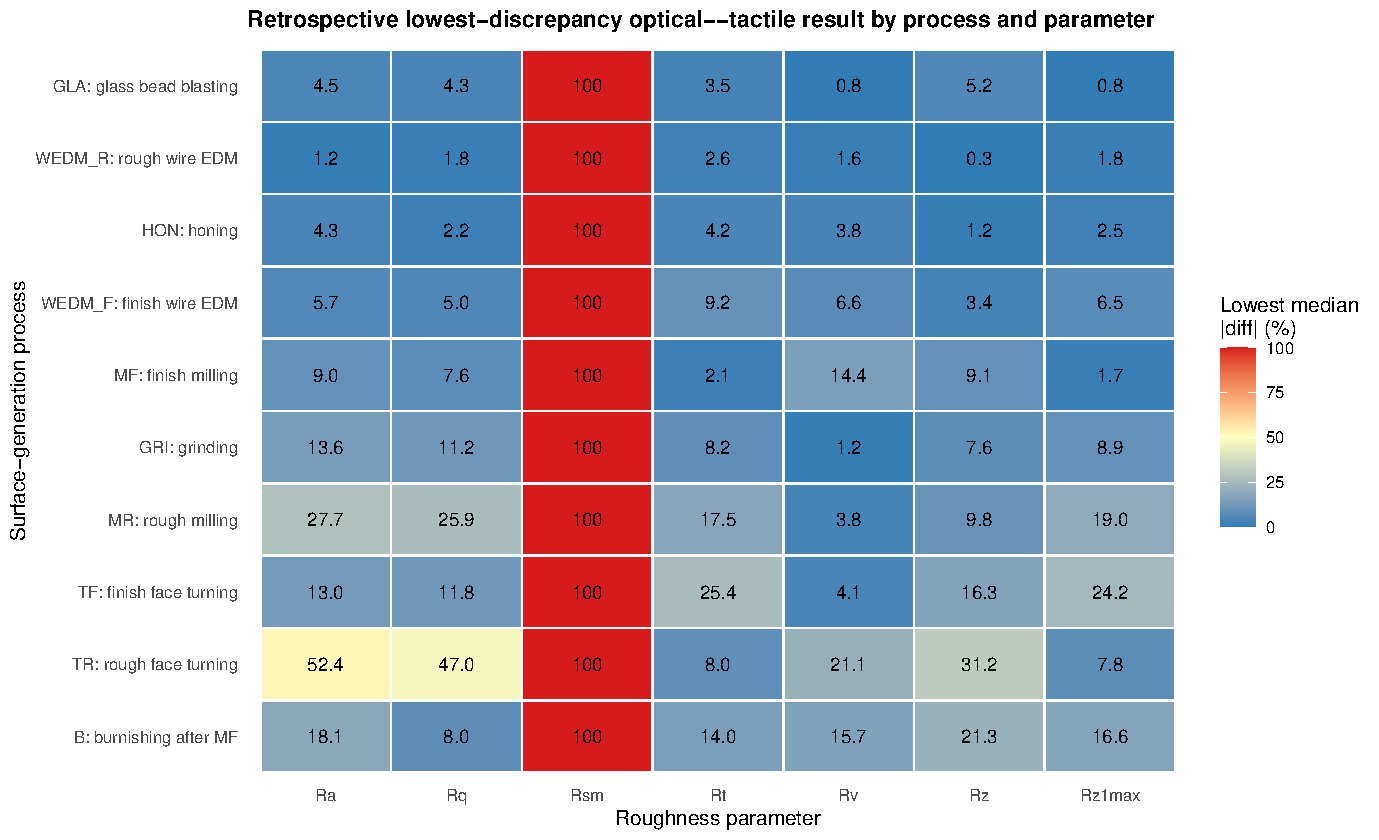
\includegraphics[width=0.98\linewidth]{../plots/global_best_discrepancy_heatmap.pdf}
  \caption{Global process--parameter map of best-achievable optical--tactile median discrepancy for the seven strictly positive roughness parameters. Values are median $|\mathrm{diff}|(\%)$ after selecting the best available system--illumination pair within each material--process--parameter group; colour scale is capped at 100\% for readability.}
	\label{fig:global_best_discrepancy_heatmap}
\end{figure}

Across the full dataset, interferometry-based measurements (\textit{int}) appear most frequently as the best-achievable configuration for most parameters, and red/green illumination bands are most often associated with the best-achievable median $|\mathrm{diff}|(\%)$ (Table~\ref{tab:decision_by_param}). However, there are process- and material-specific exceptions in which other systems, notably focus variation (\textit{FV}), become the most frequent best-achievable choice (Tables~\ref{tab:decision_by_process}--\ref{tab:decision_by_material}). These frequencies should be read as patterns within the tested archive, not as universal rankings for future applications.

Figure~\ref{fig:effects_by_system} illustrates the main effects of the measurement system on the absolute percentage error using the representative case of $R_a$ on Ti6Al4V after finish milling. Analogous plots for other material--process combinations are included in the Supplementary Materials.

\begin{figure}[H]
	\centering
	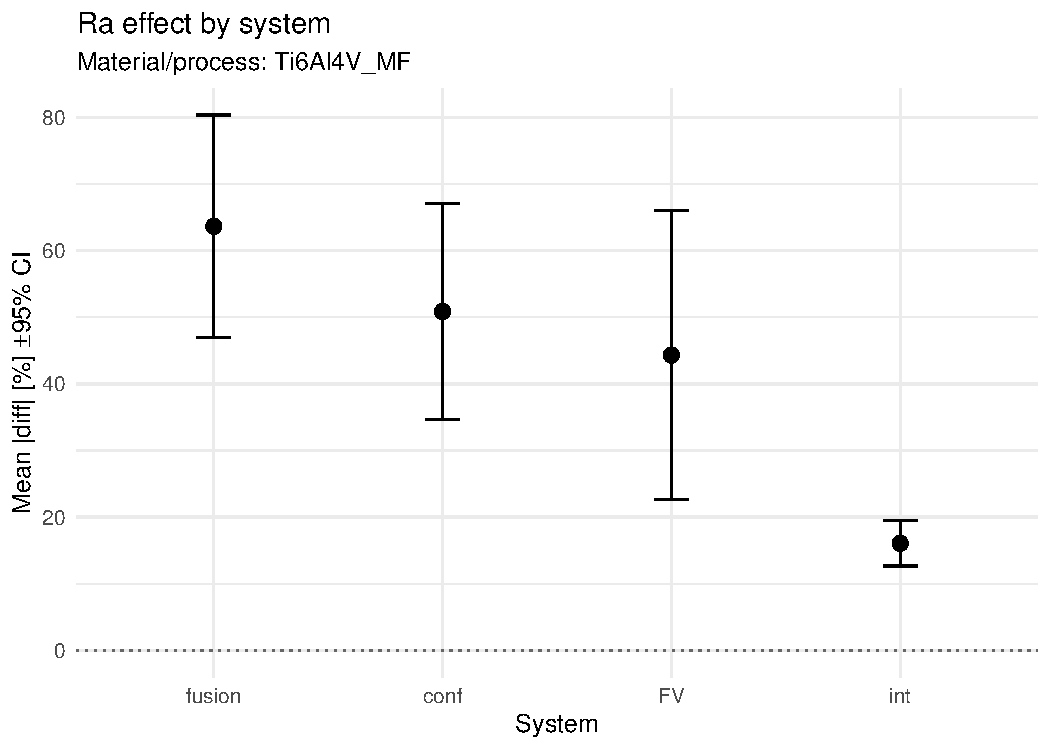
\includegraphics[width=0.9\linewidth]{../plots/ra_abs_ti6al4v_mf_effects_by_system.pdf}
  \caption{Main effects of the measurement system on absolute roughness error $|\mathrm{diff}|(\%)$ for $R_a$ on Ti6Al4V after finish milling}
	\label{fig:effects_by_system}
\end{figure}

\subsection{\texorpdfstring{Representative Example: Ti6Al4V after\\Finish Milling}{Representative Example: Ti6Al4V after Finish Milling}}
To illustrate the system-to-system variability observed across the full dataset, a detailed example is shown for Ti6Al4V after finish milling, which represents a technologically relevant, moderately smooth surface. This example should be interpreted in the context of the decision summaries above: for $R_a$, roughly half of all available material--process groups (for that parameter) can reach $\leq 10\%$ disagreement after selecting the best optical system and colour (Table~\ref{tab:decision_by_param}), while Ti6Al4V as a material is among the more challenging cases in aggregate (Table~\ref{tab:decision_by_material}).

For Ti6Al4V after finish milling, the spread of $|\mathrm{diff}|(\%)$ between systems is particularly clear. Some optical instruments yield errors close to the tactile reference under suitable illumination, whereas other configurations deviate markedly. This reinforces that optical--tactile agreement is not transferable across systems without validation and that ``optical'' must be treated as a \emph{system+illumination} choice.

Figure~\ref{fig:optics_vs_tactile} compares the distributions of $|\mathrm{diff}|(\%)$ for all optical systems against the tactile reference for Ti6Al4V after finish milling, emphasising the contrast between well-performing and outlying configurations.

\begin{figure}[H]
	\centering
	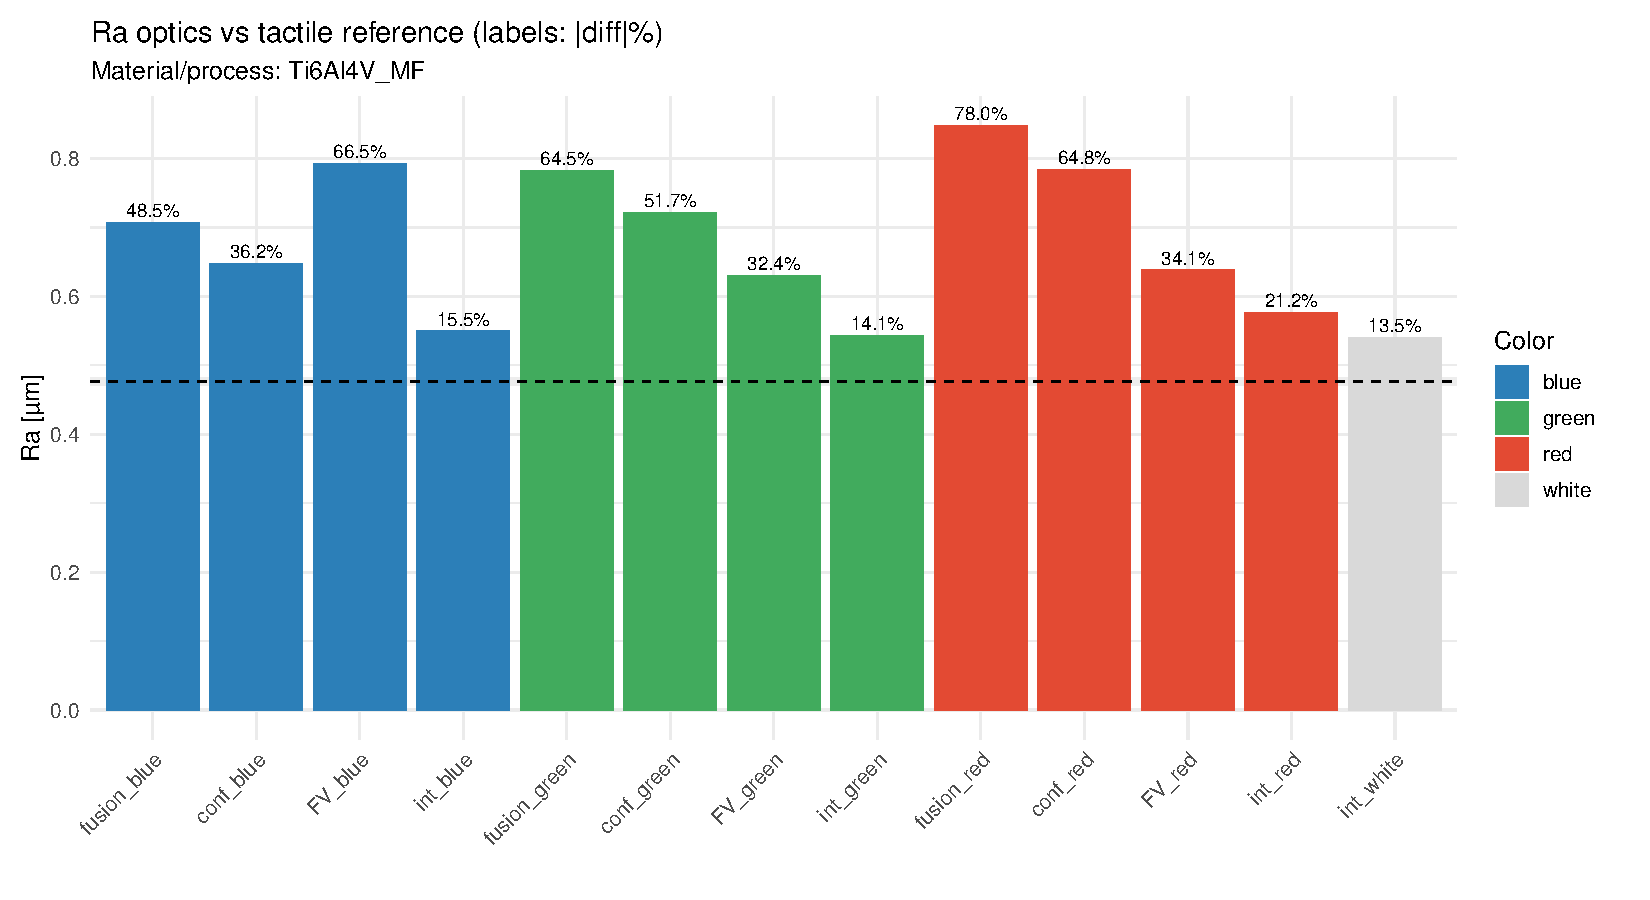
\includegraphics[width=0.9\linewidth]{../plots/ra_abs_ti6al4v_mf_optics_vs_tactile.pdf}
  \caption{Comparison of absolute roughness error $|\mathrm{diff}|(\%)$ for $R_a$ on Ti6Al4V after finish milling obtained from optical systems and the tactile reference}
	\label{fig:optics_vs_tactile}
\end{figure}

\subsection{Influence of Illumination Wavelength}
Across materials and processes, illumination colour can shift $|\mathrm{diff}|(\%)$ and, in a minority of cases, induces systematic trends with wavelength. In the full set of system-wise regressions across the analysed material--process--parameter groups, statistically significant slopes $\beta_1$ of $|\mathrm{diff}|(\%)$ versus wavelength were observed in 8.9\% of fits (203/2290), indicating that wavelength optimisation is best treated as an application-specific tuning step rather than a universal correction.\\
Because these regressions are fitted across many parameter--surface groups and typically rely on only three or four colour levels per fit, individual significant slopes should be interpreted as screening evidence; the emphasis is therefore placed on the overall rate and on patterns that replicate across systems and surfaces.

Consistent with this, ANOVA effect sizes indicate that the measurement system explains substantially more variability in $|\mathrm{diff}|(\%)$ than illumination colour for most groups (median $\eta^2_{\text{system}}=0.651$ vs. median $\eta^2_{\text{color}}=0.106$ across all ANOVA groups, $n=590$; Supplementary Table~S1). Across the same 590 parameter--surface groups, the system effect size exceeds the colour effect size in 497 cases, whereas colour exceeds system in 93. Nevertheless, colour still matters operationally because the best-achievable configuration for many parameters is tied to a specific illumination band (Table~\ref{tab:decision_by_param}), and these preferences can differ across process and material (Tables~\ref{tab:decision_by_process}--\ref{tab:decision_by_material}).

For completeness and reproducibility, the full per-group ANOVA outputs (including degrees of freedom, $F$, $p$, and $\eta^2$) are reported in Supplementary Table~S1, and the full set of system-wise wavelength-regression slopes is reported in Supplementary Table~S2. Correlation coefficients were used as a complementary descriptive diagnostic alongside regression; to avoid redundancy, the paper reports regression slopes as the primary summary. Additional system- and colour-wise effect plots supporting follow-up comparisons are provided in the Supplementary Materials.

Figure~\ref{fig:diff_vs_wavelength} shows an example of the dependence of $|\mathrm{diff}|(\%)$ on illumination wavelength for $R_a$ on Ti6Al4V after finish milling, together with fitted screening lines that illustrate the estimated trend for each optical system.

\begin{figure}[H]
	\centering
	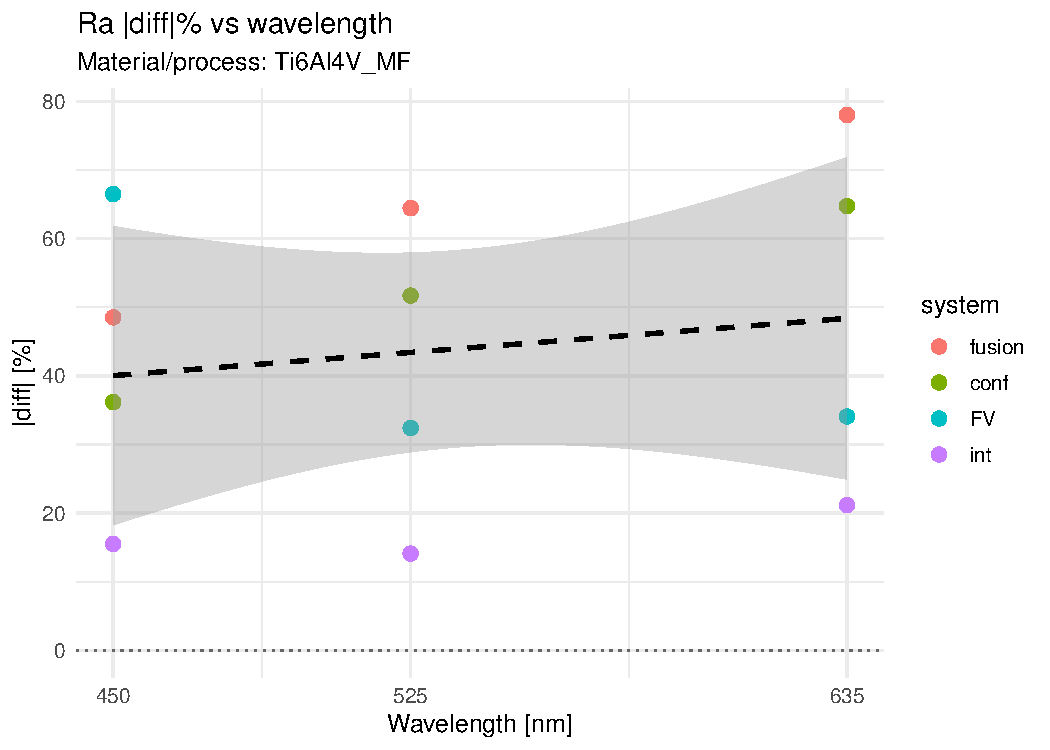
\includegraphics[width=0.9\linewidth]{../plots/ra_abs_ti6al4v_mf_diff_vs_wavelength.pdf}
  \caption{Dependence of absolute roughness error $|\mathrm{diff}|(\%)$ for $R_a$ on Ti6Al4V after finish milling on illumination wavelength for individual optical systems; lines indicate fitted screening trends}
	\label{fig:diff_vs_wavelength}
\end{figure}

\subsection{Technical Distance between Systems}
The technical distance matrix derived from mean $|\mathrm{diff}|(\%)$ highlights clusters of optical systems that behave similarly across the investigated materials and surface treatments. Systems within the same cluster tend to exhibit comparable error levels and wavelength trends, whereas isolated systems form distinct groups at large distances from the rest. This summary is descriptive: small distances indicate similar disagreement patterns within the analysed dataset, but do not by themselves establish matched metrological behaviour, shared traceability, or a common calibration strategy.\\
As a representative example, Figure~\ref{fig:tech_distance} shows the technical distance matrix for $R_a$ on Ti6Al4V after finish milling. Equivalent matrices for other material--process combinations and parameters are available in the Supplementary Materials, and they provide a compact complement to the decision tables (Tables~\ref{tab:decision_by_param}--\ref{tab:decision_by_material}) by showing which systems behave similarly \emph{within a given material--process context}.

\begin{figure}[H]
	\centering
	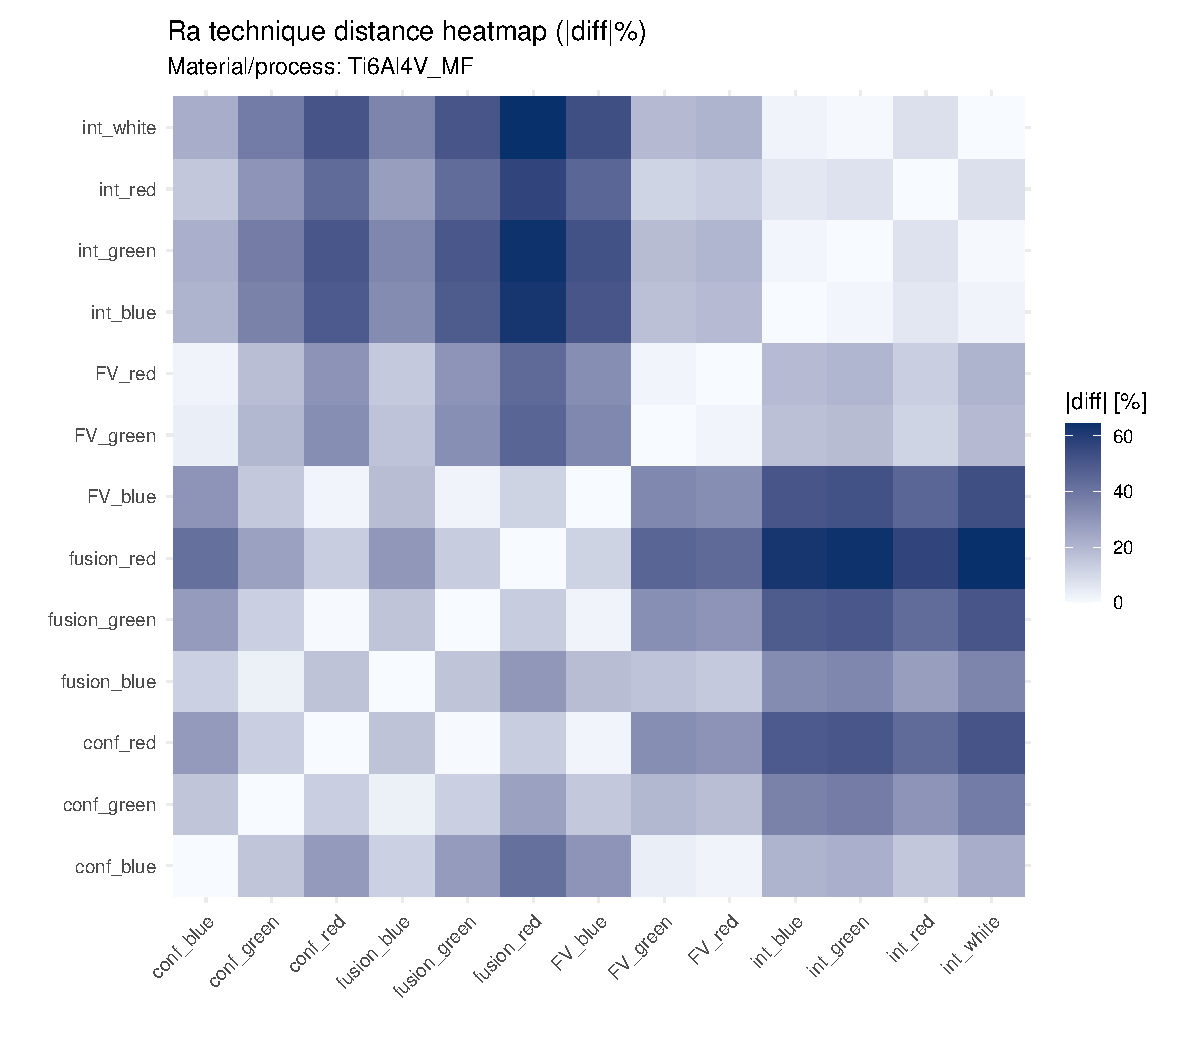
\includegraphics[width=0.9\linewidth]{../plots/ra_abs_ti6al4v_mf_tech_distance_heatmap.pdf}
  \caption{Technical distance matrix between optical and tactile systems for $R_a$ on Ti6Al4V after finish milling, based on mean absolute roughness error $|\mathrm{diff}|(\%)$}
	\label{fig:tech_distance}
\end{figure}

\section{Discussion}

A multi-material retrospective benchmark of optical workflows against an internal tactile baseline has been presented. Within the archive and its parameter-label comparison frame, three patterns are robust. First, system choice dominates the discrepancy structure across the archive. Second, illumination band matters, but mainly as a secondary, system-specific tuning variable. Third, performance is strongly parameter-dependent: amplitude-type parameters can enter a lower-discrepancy regime under selected configurations, whereas $R_{sm}$ remains difficult.

The decision tables identify the best-performing workflow observed within each parameter--surface group and are therefore best used as screening tools for follow-up validation rather than as fixed-setup performance claims. The same logic applies to the statistical summaries. The ANOVA decompositions and wavelength regressions summarise patterns in an unbalanced archive, especially where only three or four illumination levels were available, and are not intended as causal or transferable correction models. Percentage-based $R_{sk}$ summaries are retained in the archive-derived tables for completeness only and should not be interpreted on the same footing as the strictly positive parameters.

The fixed-configuration sensitivity analysis is important because it separates two different practical questions. If the task is to screen an archive and identify promising follow-up candidates, the retrospective best-achievable summaries are useful. If the task is to choose one optical setup before measurement, the fixed-workflow rows are more relevant and more conservative. The gap between the two is substantial: the best complete-coverage fixed workflow has a median discrepancy of 24.8\%, whereas several amplitude parameters achieve best-achievable medians below 10\% only after the workflow is allowed to vary by parameter--surface group. This result strengthens, rather than weakens, the benchmark interpretation: optical workflow selection is itself part of the metrological decision.

From a practical perspective, the archive supports workflow triage rather than workflow substitution. The results identify where optical configurations merit prospective testing, where system choice is decisive, and where tactile confirmation remains prudent. For laboratories using multiple instruments, the technical distance maps provide an operational summary of which workflows behave similarly within a given material--process context, but they do not imply shared calibration or metrological equivalence.

A prospective study designed to support stronger tactile--optical equivalence claims would require a narrower and more rigorous protocol than the one available here. At minimum, such a study would need matched specimen-level raw profiles, harmonised filtering and form-removal settings, within-instrument and between-instrument repeatability, and a combined uncertainty model covering both tactile and optical workflows. System and illumination settings would also need to be fixed a priori, or selected in a separate development phase, rather than retrospectively optimised on the reporting dataset.

\subsection{Study limitations}
Several limitations define the scope of the present conclusions. First, the study compares exported roughness parameters in a harmonised comparison space defined by matched material--process identifiers and same-named parameter labels, but it does not reconstruct a fully harmonised raw-profile measurand definition for every instrument pair. The reported discrepancies are therefore workflow discrepancies rather than formal measurement errors. Second, the tactile mean is an internal baseline derived from $n=20$ repeats with an available repeatability descriptor ($s_S$, $u_S$), not a certified reference value with a complete uncertainty budget, so the results should not be interpreted as traceability-qualified accuracy statements. Third, the best-achievable decision tables are retrospective because the best system+colour is selected after observing the data; the fixed-configuration sensitivity analysis quantifies this optimism but does not replace a prospective fixed-protocol validation. Fourth, wavelength regressions and the descriptive summaries in Supplementary Tables~S2--S3 are often based on only three or four colour levels per system, so they are suitable for screening trends but not for strong inference on wavelength laws or instrument physics. Fifth, raw profiles, common filtering settings, complete optical instrument metadata, and a combined tactile--optical uncertainty model were not consistently available across the archive. Finally, percentage-based $R_{sk}$ summaries are intrinsically unstable near zero and are therefore retained only as secondary screens.

\section{Conclusions}

Within these limits, the main findings of the multi-material benchmark can be summarised as follows:
\begin{itemize}
	\item \textbf{System choice is the primary driver of disagreement.} Across all analysed parameter--surface combinations, the ANOVA effect size for system is large (median $\eta^2=0.651$, interquartile range 0.357--0.831), and across the 590 parameter--surface groups with both system and colour effect sizes available, system has the larger $\eta^2$ in 497 cases (Supplementary Table~S1).
	\item \textbf{Illumination colour is secondary but non-negligible.} The ANOVA effect size for colour is much smaller (median $\eta^2=0.106$, interquartile range 0.048--0.210), and colour has the larger $\eta^2$ in 93 of the same 590 groups; thus, wavelength/colour optimisation should be treated as a system-specific tuning step rather than a universal correction.
	\item \textbf{Wavelength trends are present in a minority of cases.} Across all fitted system-wise regressions, statistically significant slopes of $|\mathrm{diff}|(\%)$ versus wavelength are observed in 8.9\% of cases (203/2290) at a nominal $\alpha=0.05$. Rates are lowest for $R_a$ (6.6\%) and higher for amplitude parameters such as $R_t$ (12.2\%), $R_z$ (11.4\%) and $R_{z1max}$ (10.9\%) (Supplementary Table~S2); these fits should be read as screening summaries because they are typically based on only three or four wavelength levels.
	\item \textbf{Parameter dependence is substantial.} Best-achievable discrepancy differs sharply across the strictly positive parameters: amplitude-type measures such as $R_t$, $R_v$, $R_z$, and $R_{z1max}$ achieve median best discrepancy of 4.8--6.6\%, $R_a$ and $R_q$ remain below 10\% in median terms, and $R_{sm}$ remains problematic at 99.9\% (Table~\ref{tab:decision_by_param}). Percentage-based $R_{sk}$ summaries are retained for archive completeness only and are not interpreted on the same footing as the strictly positive parameters. Conclusions drawn from a single parameter should therefore not be overgeneralised to others.
	\item \textbf{Retrospective selection materially improves the apparent result.} In the fixed-configuration sensitivity analysis, the best single workflow with complete coverage is interferometry with green illumination, but its median discrepancy is still 24.8\% across the 413 strictly positive parameter--surface groups (Table~\ref{tab:fixed_workflow_sensitivity}). The decision tables should therefore be used to prioritise candidate workflows for prospective validation, not to recommend one universal optical setup.
  \item \textbf{The archive supports a limited internal reference-uncertainty treatment.} Across all 472 parameter--surface groups in the manuscript subset, the tactile reference is based on $n=20$ repeats. For the seven strictly positive parameters, the relative standard error of the tactile mean has median 1.45\% (Q1--Q3 0.85--2.44\%), indicating that tactile repeatability is typically smaller than the observed optical disagreements.
	\item \textbf{The main output is a benchmark for follow-up selection, not a universal setup recommendation.} The decision summaries capture the lowest disagreement observed within the tested system+colour combinations for each parameter--surface group, so they are best used to prioritise candidate optical workflows for prospective validation. They do not represent the performance of a single fixed setup, nor do they establish full tactile/optical equivalence.
\end{itemize}

Overall, the study identifies where lower optical--tactile discrepancy was observed within the tested configurations and where tactile confirmation remained preferred. Its main contribution is a practical benchmark for selecting candidate optical workflows and prioritising follow-up validation.

\section*{Acknowledgments}
The authors gratefully acknowledge the support of the Polish Ministry of Science. This work was funded by grant PM-II/SP/0090/2024/02.


\section*{Supplementary Materials}
The following supporting information is available online at the journal website:
\begin{itemize}
  \item \textbf{Supplementary S1}: additional tables and figures extending the Results. The material includes (i) two-way ANOVA main effects and $\eta^2$ effect sizes for the factors system and colour (Supplementary Table~S1), (ii) system-wise slopes of $|\mathrm{diff}|(\%)$ versus illumination wavelength (Supplementary Table~S2), (iii) descriptive statistics by system (Supplementary Table~S3), and (iv) parameter-wise internal tactile repeatability summaries (Supplementary Table~S4), together with additional plots for selected material--process combinations.
\end{itemize}

\section*{Conflicts of Interest}
The authors declare no conflict of interest.\\
\noindent\textbf{Funding:} This work was supported by a grant from the Polish Ministry of Science under the programme “Polish Metrology II” (Polska Metrologia II, Poland), project no. PM-II/SP/0090/2024/02. 

\section*{Data Availability}
The R/Python analysis scripts, configuration files, manuscript and supplement sources, generated CSV outputs, generated tables, and generated figures supporting the findings are provided in a public GitHub repository: \url{https://github.com/dawidkucharski/optical-tactile-surface-benchmark}. Raw \texttt{.sur} surface files are excluded from the public repository because they are original instrument exports and may be large or restricted, but the derived CSV outputs needed to reproduce the manuscript tables, fixed-workflow sensitivity analysis, global heatmap, and supplementary tables are included. The excluded raw \texttt{.sur} files are available from the authors on reasonable request, subject to data-transfer constraints. A versioned DOI release is recommended for the submitted repository snapshot.

% References are supplied via BibTeX; set style as needed for the target journal.
%\bibliographystyle{elsarticle-num}
\bibliographystyle{unsrt}
\bibliography{bibliography}

\end{document}